%Settings {{{
\documentclass[final]{beamer}
\usepackage[orientation=portrait,size=a0,scale=1,debug]{beamerposter}
\usepackage[T1]{fontenc}
\usepackage{lmodern}
\usetheme{gemini}
\usecolortheme{ox}
\usepackage{graphicx}
\usepackage{booktabs}
\usepackage{tikz}
\usepackage{pgfplots}
\pgfplotsset{compat=1.14}
\usepackage{anyfontsize}

%\setsansfont{FoundSteBoo}
%default font setup for use with pdflatex
%\renewcommand{\rmdefault}{phv} %%% Helvetica (very similar to Arial)


% ====================
% Lengths
% ====================

% If you have N columns, choose \sepwidth and \colwidth such that
% (N+1)*\sepwidth + N*\colwidth = \paperwidth
\newlength{\sepwidth}
\newlength{\colwidth}
\setlength{\sepwidth}{0.025\paperwidth}
\setlength{\colwidth}{0.3\paperwidth}

\newcommand{\separatorcolumn}{\begin{column}{\sepwidth}\end{column}}

\footercontent{

\begin{minipage}{0.33\linewidth}
~[1] O. Băzăvan et al., Phys. Rev. A, vol. 107, no. 2, p. 022617  \\\vspace{0.1em}
[2] V. M. Schäfer et al., Nature, vol. 555, no. 7694, Art. no. 7694,
\end{minipage}
\begin{minipage}{0.31\linewidth}
  \centering
  \href{mailto:donovan.webb@physics.ox.ac.uk}{donovan.webb@physics.ox.ac.uk}\\
SAMOP 2023
\end{minipage}
\begin{minipage}{0.33\linewidth}
  \hfill
  \colorbox{white}{
\includegraphics[height=3.5cm]{figs/NPL-logo.png}}~~~
  
\includegraphics[height=3.5cm]{figs/ARO-logo.png}~~~
  \colorbox{white}{
\includegraphics[height=3.5cm]{figs/QCS-logo.pdf}}
\end{minipage}
}

% ====================
% Logo (optional)
% ====================

% use this to include logos on the left and/or right side of the header:
% \logoright{
\includegraphics[height=7cm]{logo1.pdf}}
\logoleft{\fbox{
    
\includegraphics[height=9cm]{figs/oxlogo.pdf}}
}

\newcommand{\SubItem}[1]{
    {\setlength\itemindent{15pt} \item[] #1}
}

%}}}

%title {{{

\title[FastGates]{\Huge Next generation platform for implementing fast gates in ion trap quantum computation}
\author{D. Webb \and S. Saner \and O. Bazavan \and M. Minder \and C.J. Ballance\phantom{**}}
\institute[]{
Ion Trap Quantum Computing Group,
Department of Physics, University of Oxford}

\begin{document}
\begin{frame}{} 
%}}}

\begin{center}

%Abstract {{{

    \vspace{-1em}
    \begin{block}{}
    \large
    Scalable trapped-ion quantum computation relies on the development of
    high-fidelity fast entangling gates in a many ion
    crystal. Conventional geometric phase gates either suffer from
    scattering errors or off-resonant carrier excitations. A potential
    route to achieve fast entanglement is creating a standing wave which
    can suppress the unwanted carrier coupling. \\

    %% We present the roadmap to our next-generation platform tailored for
    %% fast gates in the ~1us regime where gate speeds become comparable to
    %% the secular trap frequency. The quadrupole transitions between S1/2
    %% and D5/2 levels in Calcium 40 will be driven to perform
    %% Molmer-Sorenson gates with a standing wave rather than a typical
    %% travelling wave. The off-resonant carrier excitation may be strongly
    %% suppressed by placing ions at the nodes of the optical lattice. This
    %% new platform has scope for a multi-ion chain and a corresponding array
    %% of optical lattices which each address a single ion. The lattice array
    %% is created by a set of counter-propagating beams which are tightly
    %% focused by a symmetric setup of high-NA lenses. Control of the optical
    %% phase at the ion site will be achieved by actively stabilising the
    %% counter-propagating beam interferometer and feedbacking on the ion
    %% signal.
    \end{block}
%}}}

\begin{columns}[t]
  \begin{column}{0.49\textwidth}

%Why {{{
    \begin{alertblock}{Non-Adiabatic Mølmer Sørenson Gates}
      \begin{minipage}{0.83\linewidth}
      \begin{itemize}
      \item Two qubit gates are implemented by coupling spin with shared motion of the ions.
      \item Fast entangling gates enable deeper quantum computational circuit depths for given level of incoherent error.
      \item But going fast excites multiple motional modes (``spectator modes'') which can introduces errors.
      \item Mølmer Sørenson (MS) interaction is common two-qubit gate which requires a
      bichromatic field incident on the ions. Using travelling
      waves gives the Hamiltonian
      \end{itemize}
      \end{minipage}
      \begin{minipage}{0.14\linewidth}
      \begin{figure}
        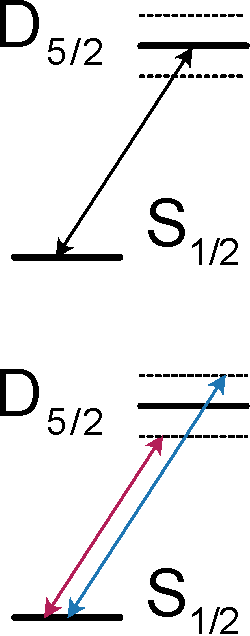
\includegraphics[width=0.7\textwidth]{./figs/level_structure.pdf}
      \end{figure}
      \end{minipage}
      \Large$$ \hat{H}_{MS-TW} = \hbar\Omega \hat{S}_{\phi-\pi/2}\cos{(\delta t)} + \hbar\Omega\eta \hat{S}_\phi\cos{(\delta t)}(\hat{a}e^{-i\omega_zt} + \hat{a}^\dagger e^{i\omega_zt})$$\normalsize
      \vspace{0.4em}
      with the first term being the carrier whilst the second is the desired coupling.
      \begin{itemize}
      \item As these terms do not commute, in the interaction picture this Hamiltonian
            may be expressed as [1]:
      \Large$$ \hat{H}_{MS-TW} = \hbar\eta\Omega(J_0(2\Omega/\delta) + J_2(2\Omega/\delta))\cdot \cos{(\delta t)}\hat{S}_{\phi}(\hat{a}e^{-i\omega_zt} + \hat{a}^\dagger e^{i\omega_zt})$$\normalsize
      \end{itemize}
      \begin{minipage}{0.58\textwidth}
      \begin{itemize}
      \item \textbf{Carrier term:} causes the spin dependent force
        coupling to be modulated by (J0+J2).

      \item \textbf{Spectator excitation:} Amplitude shaped pulses
        [2] effectively remove ``spectator'' error by closing
        phase loops of all excited modes.
        
      \end{itemize}
      \end{minipage}
      \begin{minipage}{0.38\textwidth}
      \begin{figure}
        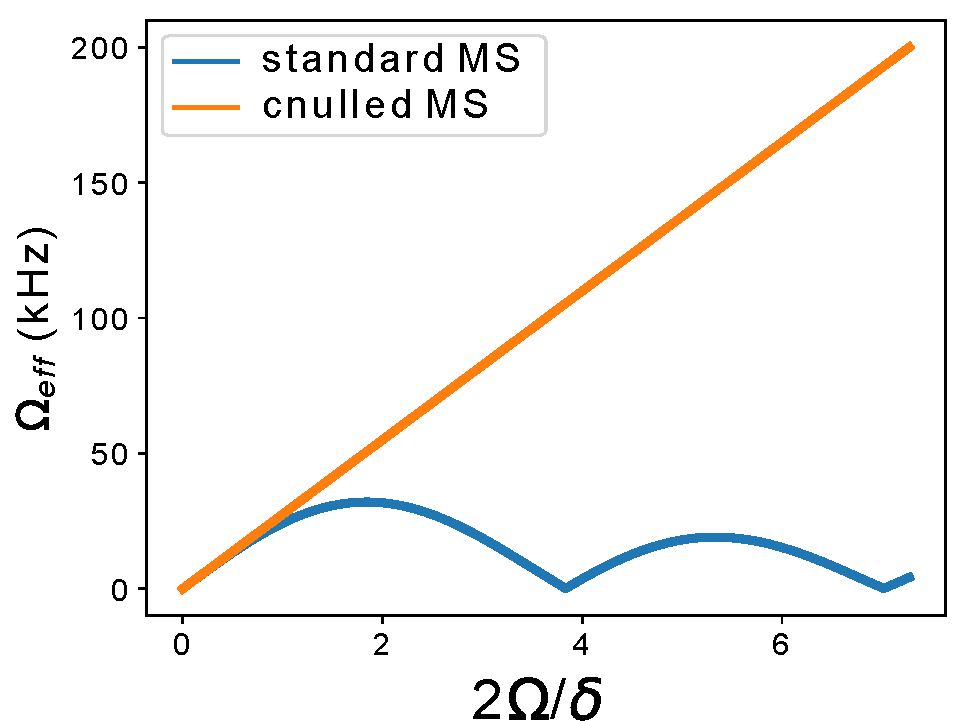
\includegraphics[width=0.7\textwidth]{./figs/J0J2theory.pdf}
        %XXX CANZZ aside box
      \end{figure}
      \end{minipage}
      \begin{figure}
        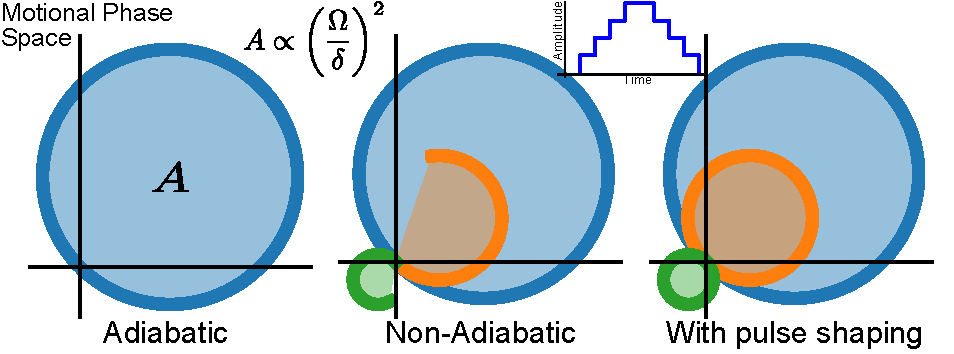
\includegraphics[width=0.7\textwidth]{./figs/phase_loops_fig.pdf}
      \end{figure}

%}}}

%Lattice {{{
    \heading{Standing Wave Single and MS Gates}
      \begin{itemize}
      \item Using standing wave gives complete control over phase
        visible to ions.
      \item This extra freedom allows fast gates by preventing the
        saturation effect seen in the travelling MS.
      \item Bichromatic standing wave Hamiltonian where ions are
        seperated by $n\lambda/2$:
      \large$$ \hat{H}_{MS-SW} = \hbar 2\Omega \hat{S}_{\phi}\cos{(\delta t)}\sin{(\Delta\phi/2)} + \hbar 2\Omega\eta \hat{S}_\phi\cos{(\delta t)}(\hat{a}e^{-i\omega_zt} + \hat{a}^\dagger e^{i\omega_zt})\cos{(\Delta\phi/2)}$$\normalsize
      \begin{figure}
        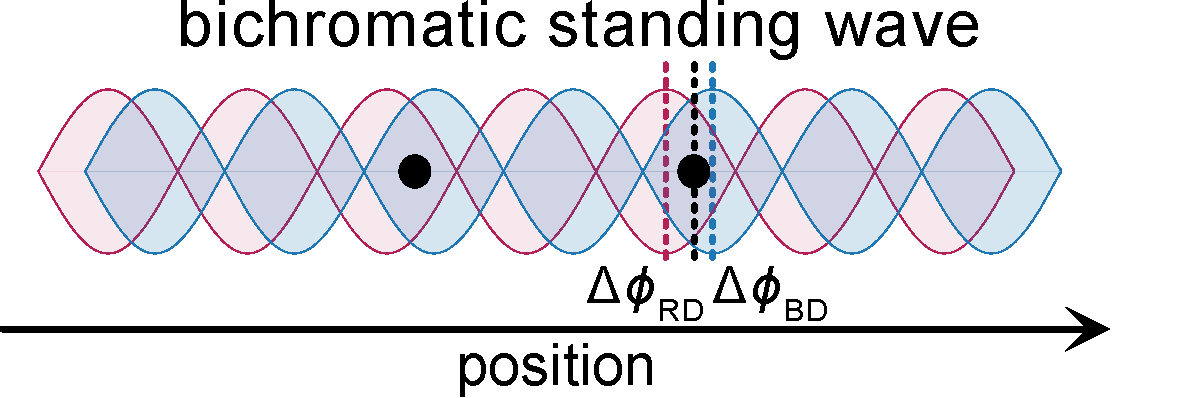
\includegraphics[width=0.8\textwidth]{./figs/bichro.pdf}
      \end{figure}
      \item Setting $\Delta\phi = 0$ (ions sitting at antinodes) we
        suppress the carrier term and maximise sideband
        coupling.
      \item However standing waves require phase stabilisation to perform
            coherent interactions.
      \end{itemize}
    \end{alertblock}
%}}}

%Phase stabilization {{{
    \begin{alertblock}{Phase Stabilization}
      \begin{minipage}{0.47\linewidth}
      \begin{figure}
        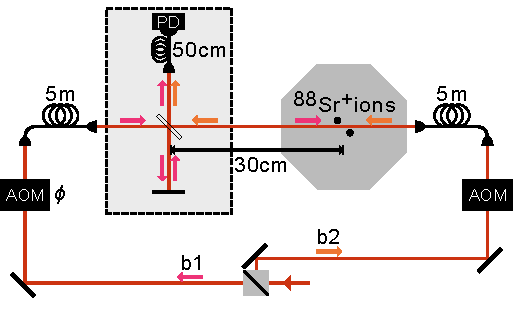
\includegraphics[width=1.05\textwidth]{./figs/setup+beams_horizontal_poster.pdf}
      \end{figure}

      \end{minipage}
      \begin{minipage}{0.53\linewidth}
      \begin{itemize}
      \item Passively using enclosure and actively by feedback process to AOM.\\
      \SubItem 1) Fast drifts removed utilising interference of light
            from the two branches on a photodiode (PD).\\

      \SubItem 2) Ion used as phase
            sensor to feedback onto an AOM ($\pi/2$ pulse on b1 and b2). \\

      \begin{figure}
        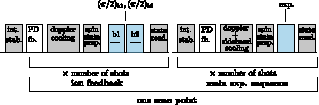
\includegraphics[width=0.94\textwidth]{./figs/beam_seq.pdf}
      \end{figure}

      \end{itemize}
      \end{minipage}
    \end{alertblock}
%}}}

%Experimental {{{
  \end{column}
  \begin{column}{0.49\textwidth}
    \begin{alertblock}{Carrier Nulling Results}
      \begin{minipage}{0.6\linewidth}
      \begin{itemize}
        \item Experimental demonstration with \textsuperscript{88}Sr\textsuperscript{+} and $674$~nm laser.
        \item Phase stability of standing wave to $\lambda/50$.
        \item Standard Randomized Benchmarking of single qubit
          rotations found gate errors of $\epsilon = 0.173(3)\%$ for
          travelling wave, $\epsilon = 0.144(3)\%$ for standing
          wave.
        \item Universal gate set with phase stabilised standing-waves.
        \item Standing wave MS maintains $>95\%$ fidelity at short gate durations in contrast to travelling wave MS sharp drop off at $\sim 25\mu s$.\\
      \begin{figure}
        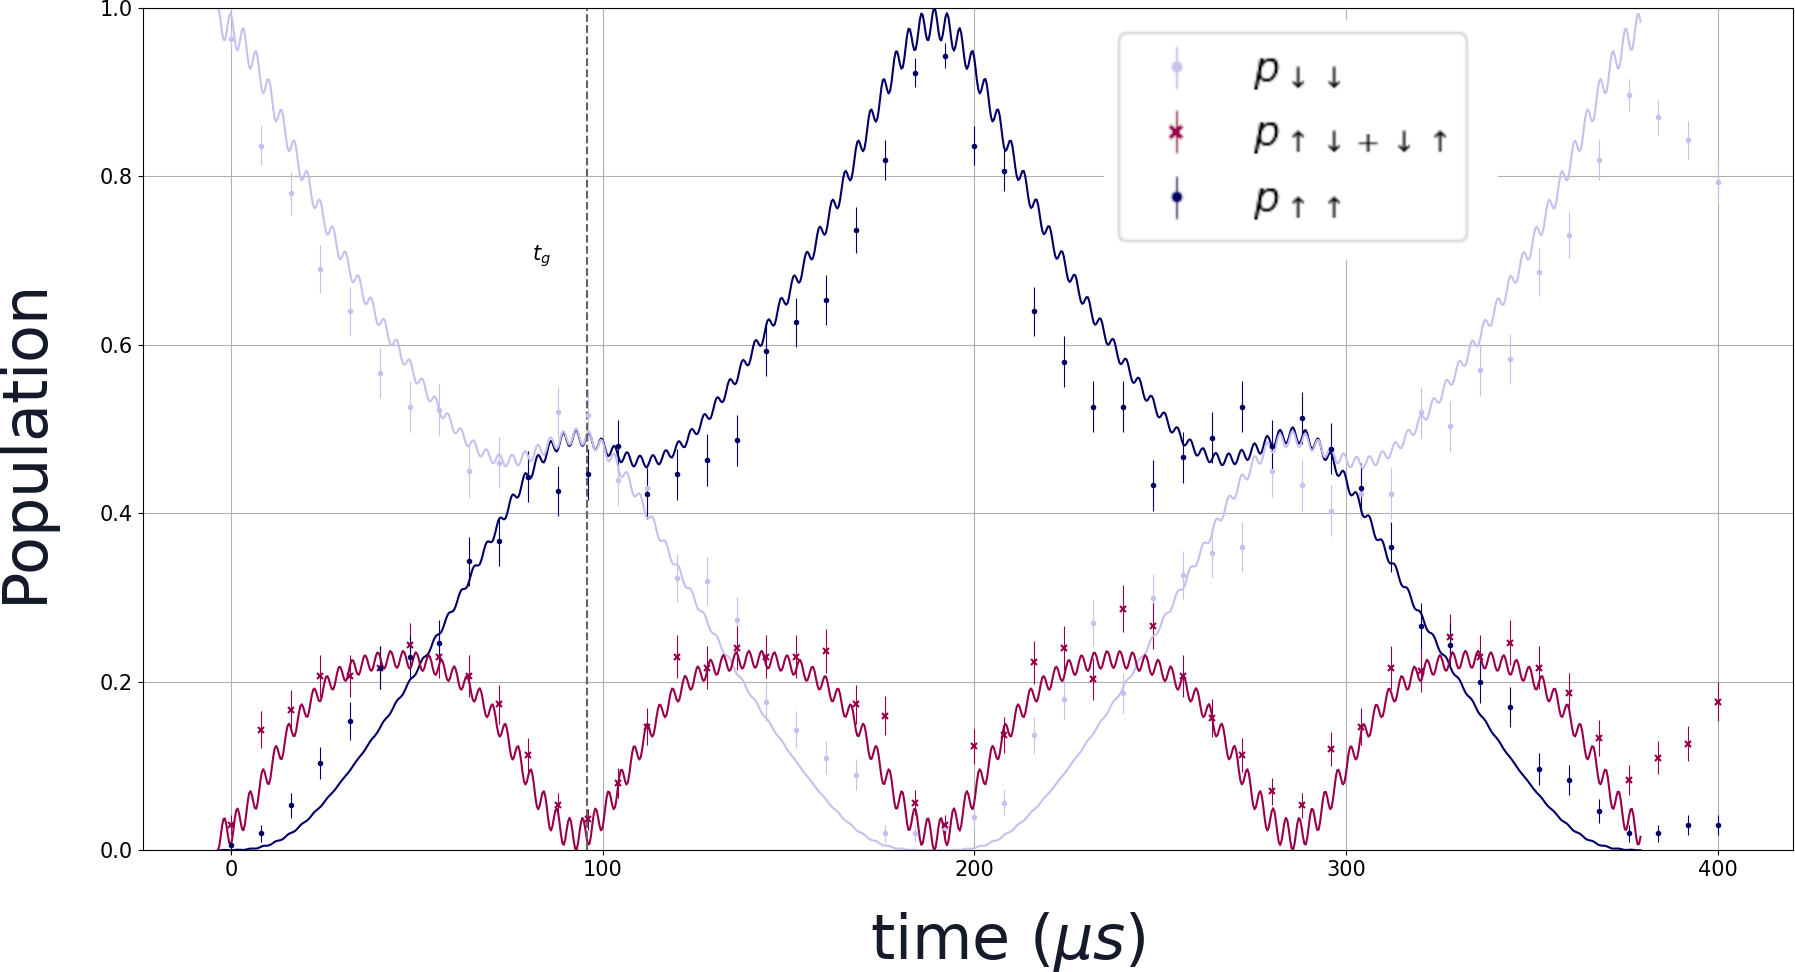
\includegraphics[width=0.7\textwidth]{./figs/temp_gate_profile.png}
      \end{figure}
      \end{itemize}
      \end{minipage}
      ~~~~
      \begin{minipage}{0.34\linewidth}
      \begin{figure}
        \fbox{
        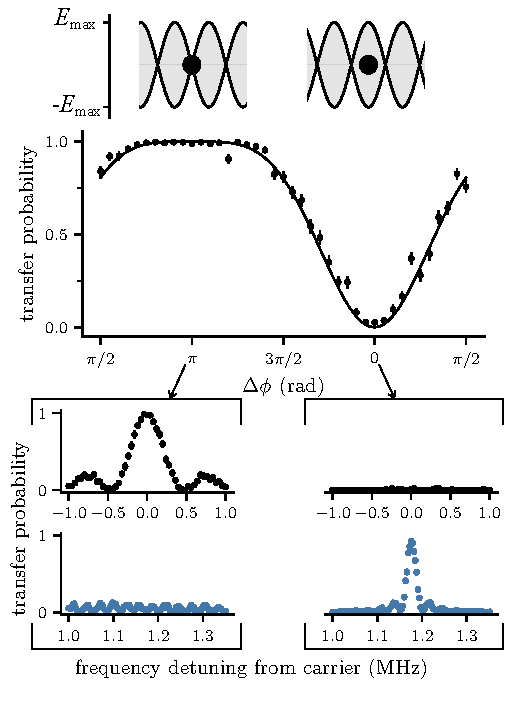
\includegraphics[width=\textwidth]{./figs/Figure_2_v2.pdf}
        }
      \end{figure}
      \end{minipage}
      \begin{figure}
        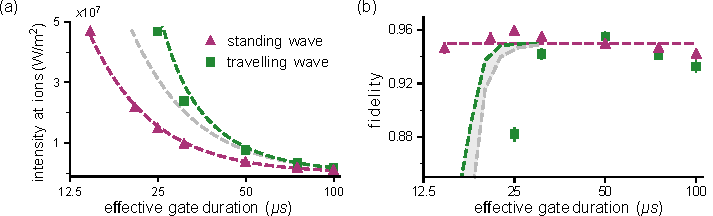
\includegraphics[width=0.8\textwidth]{./figs/two_qubit_gate_figure_h.pdf}
      \end{figure}
    \end{alertblock}


    \begin{alertblock}{New Platform}
      \begin{minipage}{0.58\textwidth}
      \begin{itemize}
      \item New \textsuperscript{40}Ca\textsuperscript{+} ion trap experiment in development for exploring fast
        gate regime using $729$~nm quadropole laser.
      \item Two high NA lenses create an array of singly
        addressing standing waves.
      \item 3D segmented trap design from NPL facilitates low heating
        rates (expected: $<10$ q/s @ $1.5$ MHz) whilst enabling ion shuttling and crystal rotations.
      \item MuMetal shield and permanent magnets for stable $B$ field.
      \end{itemize}
      \end{minipage}
      ~~
      \begin{minipage}{0.35\textwidth}
      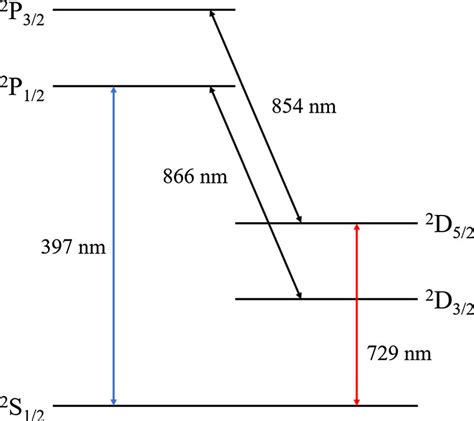
\includegraphics[width=0.94\textwidth]{./figs/ca_struct_tmp.jpeg}
      \end{minipage}

      \begin{figure}
        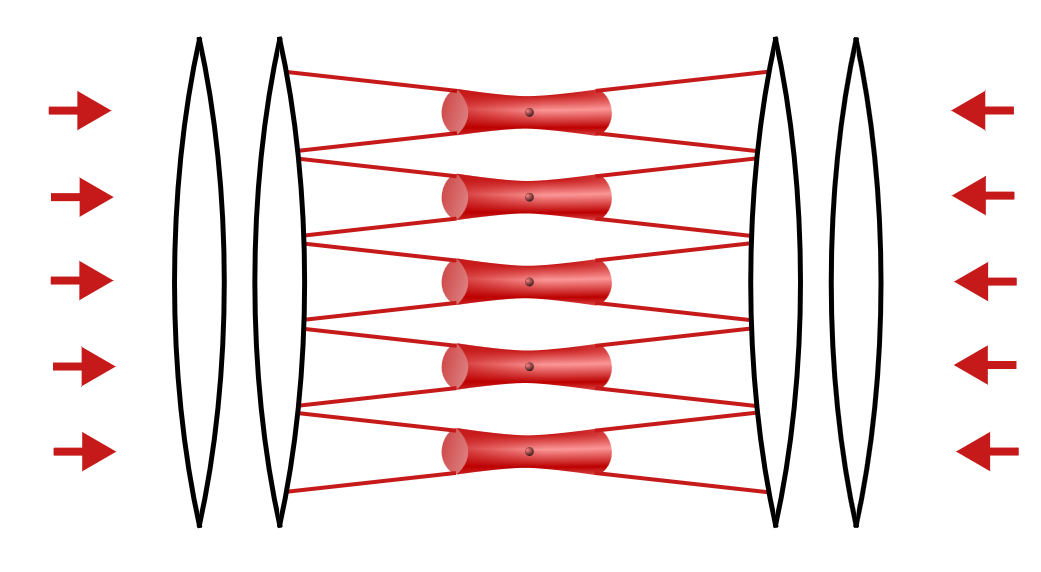
\includegraphics[height=0.285\textwidth]{./figs/array_sw.png}
        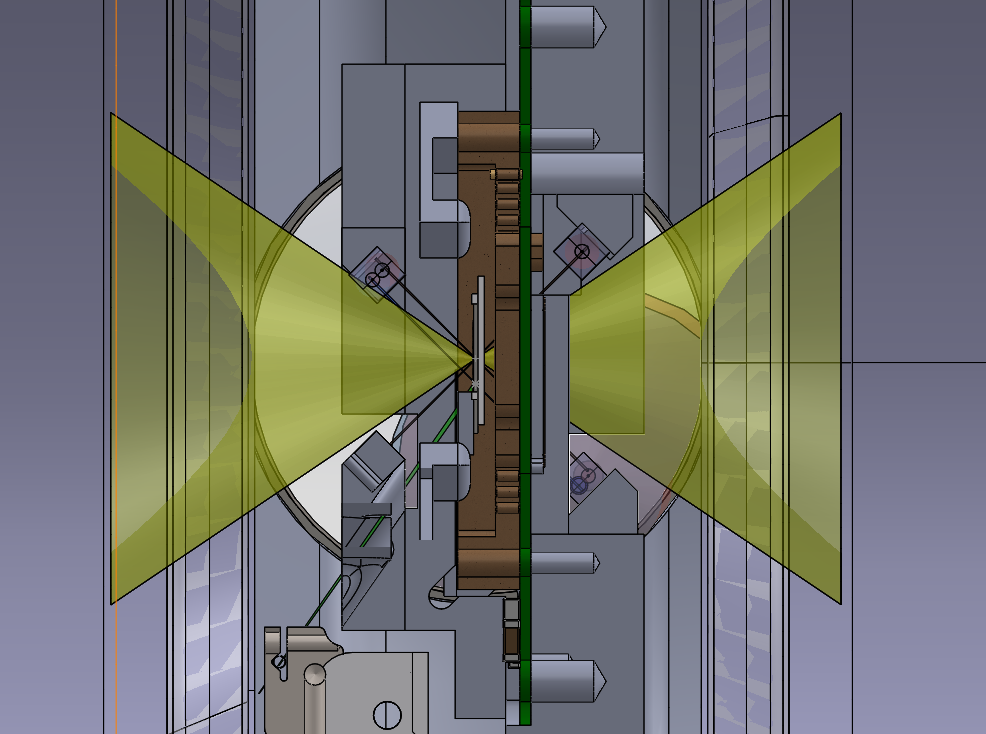
\includegraphics[height=0.285\textwidth]{./figs/trap_NA.png}\\
        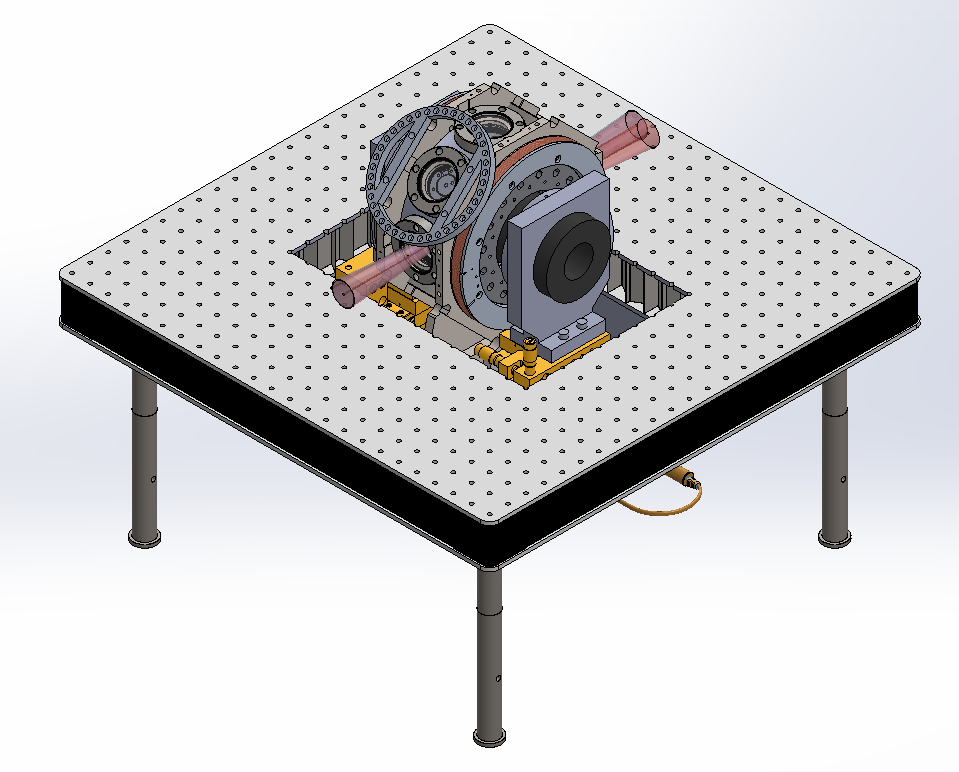
\includegraphics[height=0.35\textwidth]{./figs/exp_iso.png}
        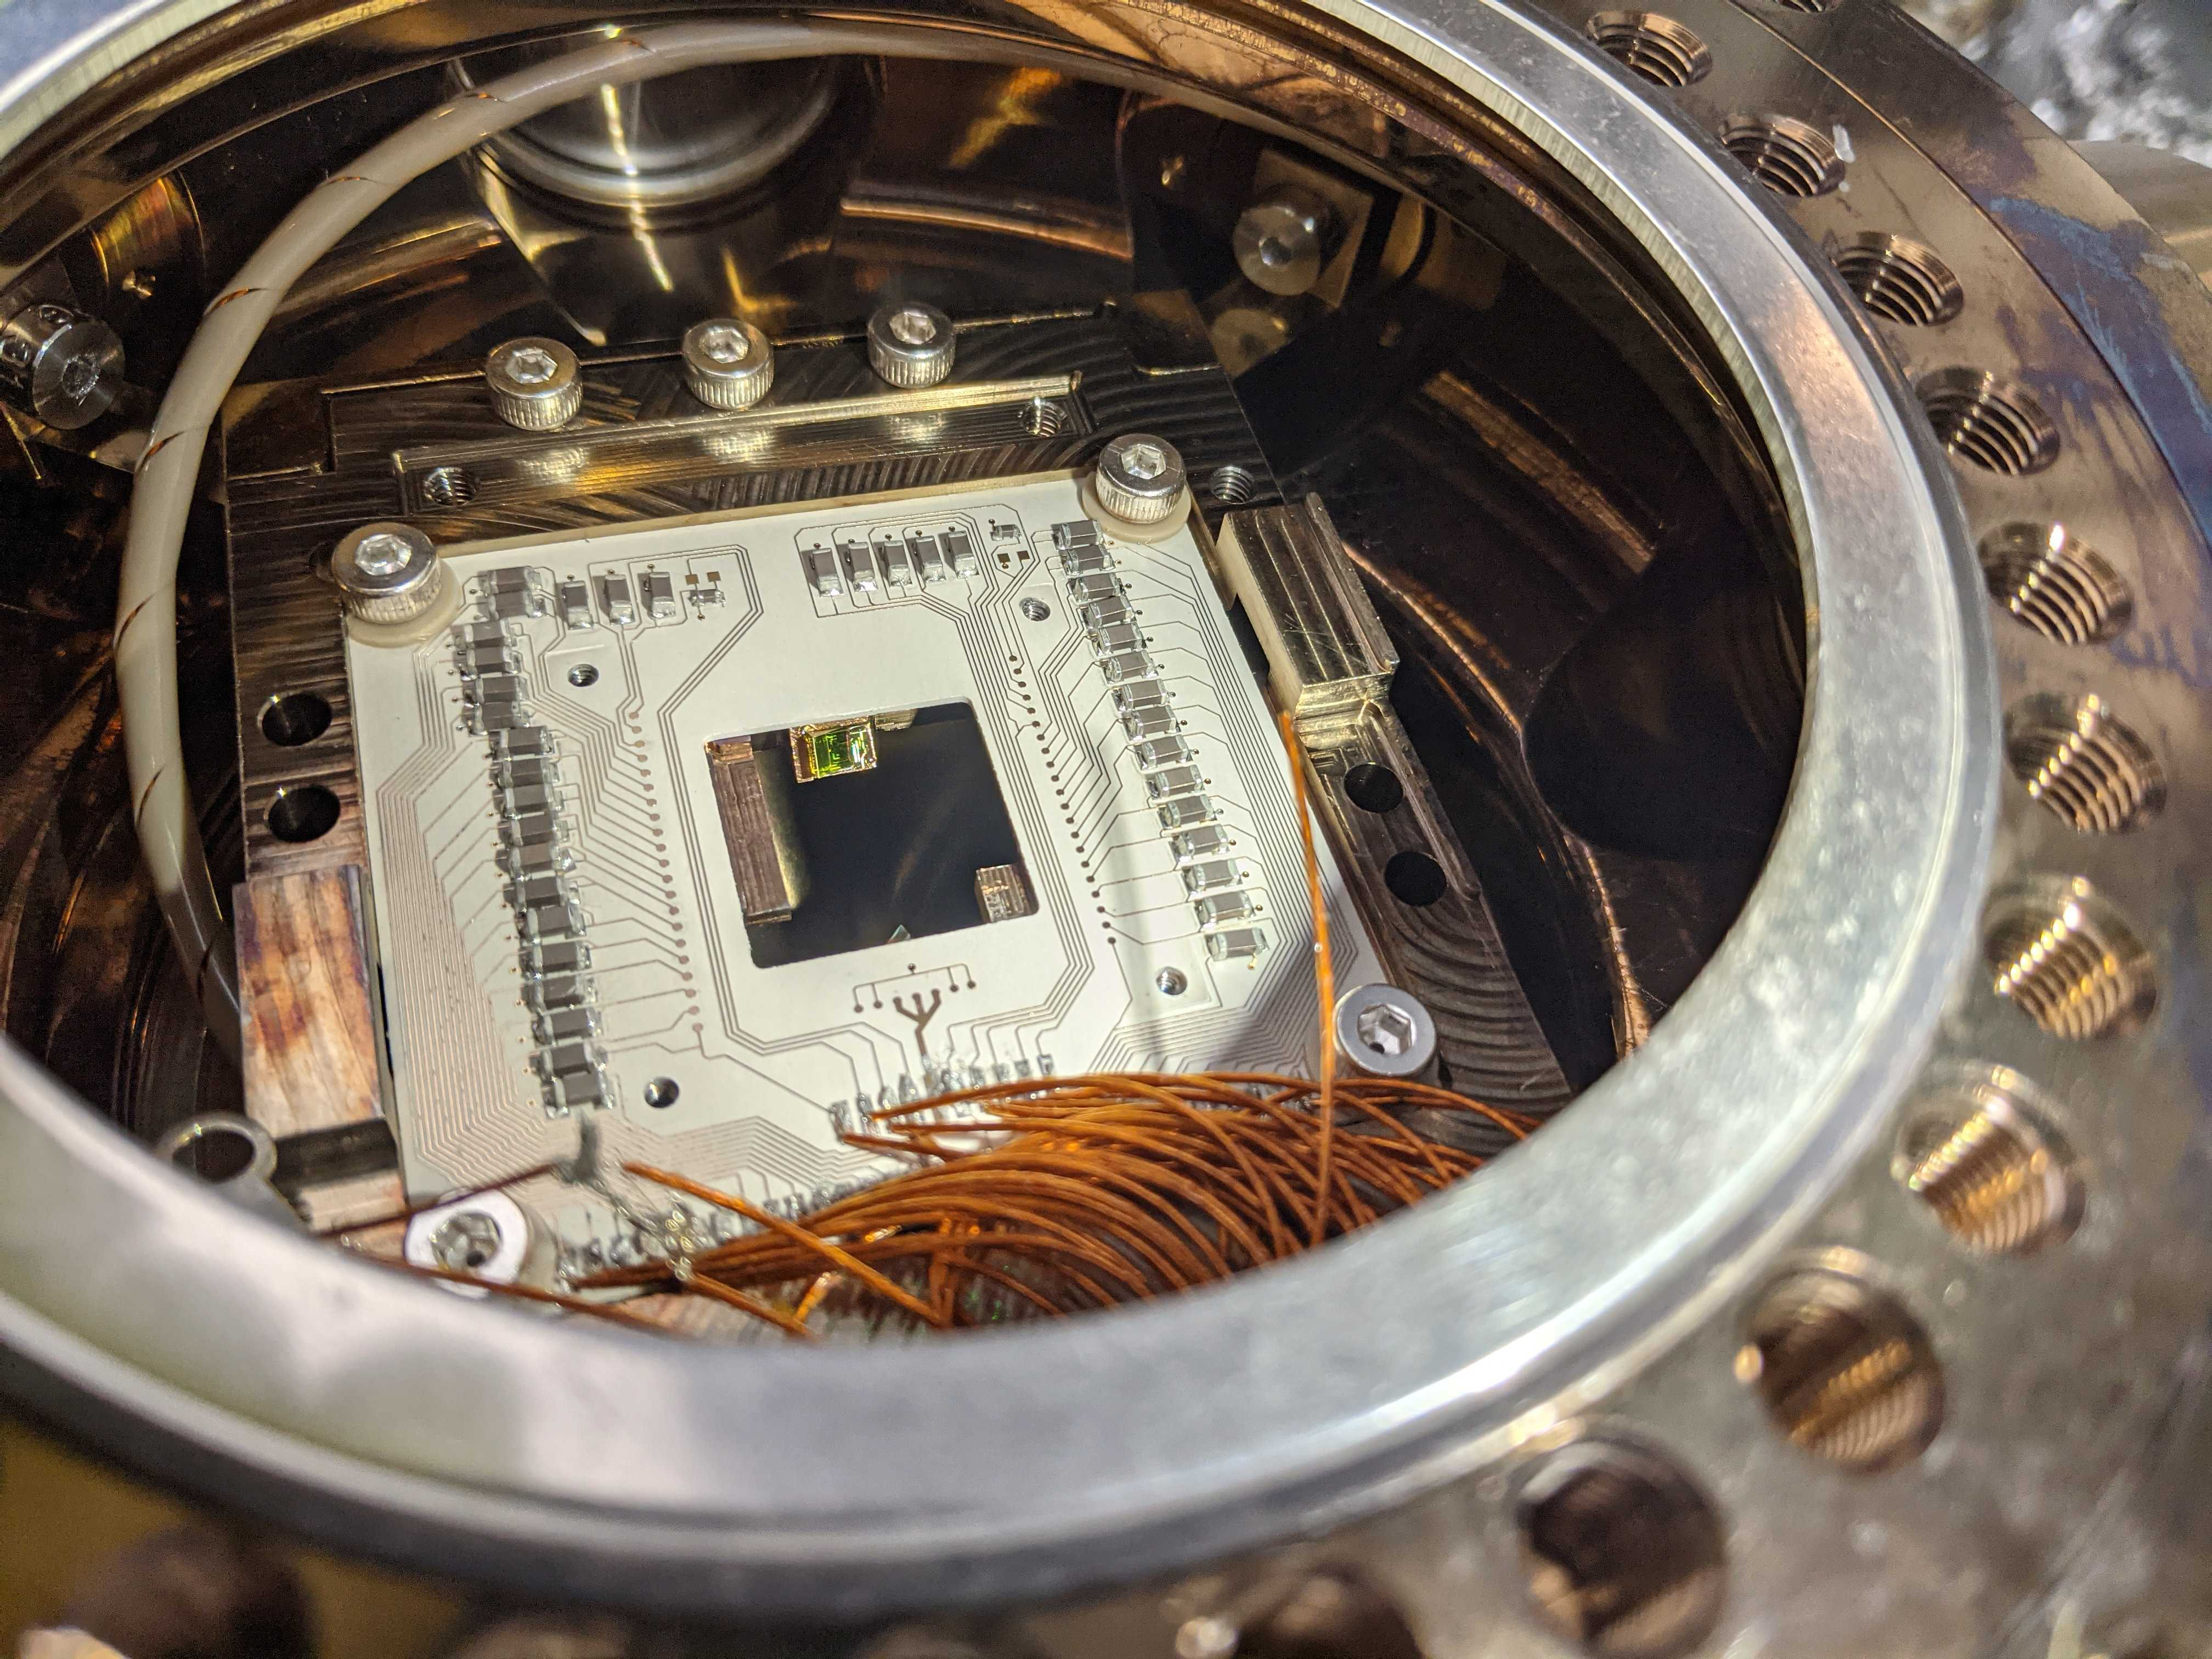
\includegraphics[height=0.35\textwidth]{./figs/mirror_photo.jpg}
      \end{figure}

    \end{alertblock}
%}}}

  \end{column}
\end{columns}

\end{center}
\end{frame}
\end{document}
